% Use for better looking tables
%\usepackage{booktabs}
%Forces tables to appear after the text that defines them
\usepackage{flafter}

%
% Index creation
%
% delete next three lines and replace newcommands with below to only have one index
% and fix hyperlinks
%

\usepackage{imakeidx}
\makeindex[intoc=true]
\makeindex[name=data,title=Index of Data Sets and Packages,intoc=true]

\newcommand{\indexpackage}[1]{\index[data]{#1 package}\index{#1 (R package)}}
\newcommand{\indexdata}[2]{\index[data]{#1 (#2)}\index{#1 (#2)}}
\newcommand{\indexfosdata}[1]{\index[data]{#1 (fosdata)}\index{#1 (fosdata)}}

%
% \newcommand{\indexpackage}[1]{\index{#1}\index{#1 (R package)}}
% \newcommand{\indexdata}[2]{\index{#1 (#2)}\index{#1 (#2)}}
% \newcommand{\indexfosdata}[1]{\index{#1 (fosdata)}\index{#1 (fosdata)}}
%

%
% The enumitem package improves itemize and enumerate lists
% just by using it.
% The most important reason to use it is
% so that exercises that begin with parts a. b. etc are formatted
% properly.
% Also, we want definition environments to have the term
% on a line by itself, followed by the definition on the next line.
%
\usepackage{enumitem}
\setdescription{style=nextline}
%\setlist[enumerate]{topsep=0pt}

% Package for custom list of tables/figures
% We use it for our image credits
\usepackage{tocloft}
\newlistof{photocredits}{photocredit}{Photo Credits}
\newcommand{\photocredit}[1]{\addcontentsline{photocredit}{photocredit}{Chapter \protect\numberline{\thesubsubsection} #1}}

%
% DRAFT watermark
%
%\usepackage{draftwatermark}

%
% QR codes for URLs
%
\usepackage{qrcode}

%
% Define block structures
%

%
% We're not using amsthm because ntheorem is more flexible
%
\usepackage{ntheorem}

% For some reason, krantz.cls eats the whitespace before theorem environments.
% This fixes it manually.
\newlength{\pretheoremskiplen}
\setlength{\pretheoremskiplen}{10pt}

% Theorem and other mathy statements
\theoremstyle{plain}
\theorembodyfont{\itshape}
\theorempreskip{\pretheoremskiplen}
\theoremseparator{.}
\newtheorem{theorem}{Theorem}[chapter]
\newtheorem{lemma}{Lemma}[chapter]
\newtheorem{corollary}{Corollary}[chapter]
\newtheorem{proposition}{Proposition}[chapter]
\newtheorem{conjecture}{Conjecture}[chapter]

% Assumptions
\theoremstyle{break}
\theorembodyfont{\itshape}
\theorempreskip{\pretheoremskiplen}
\newtheorem{assumptions}{Assumptions}[chapter]

% Definition
\theoremstyle{plain}
\theorembodyfont{\upshape}
\theorempreskip{\pretheoremskiplen}
\newtheorem{definition}{Definition}[chapter]

% Example
\theoremstyle{plain}
\theorembodyfont{\upshape}
\theorempreskip{\pretheoremskiplen}
\newtheorem{example}{Example}[chapter]

% Remark
\theoremstyle{nonumberplain}
\theorempreskip{\pretheoremskiplen}
\theorembodyfont{\upshape}
\newtheorem{remark}{Remark}

% Alert
\newenvironment{alert}%
   {%
      \vspace{4pt}\begin{leftbar}%
      \hspace{-1.5cm}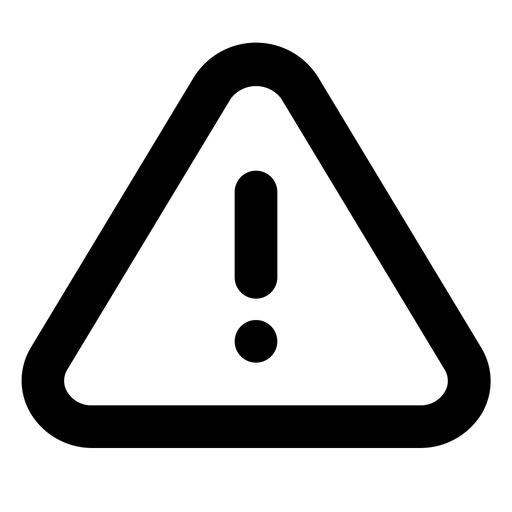
\includegraphics[height=0.8cm]{images/alert.png}%
      \vspace{-1cm}%
   }%
  {\vspace{2pt}\end{leftbar}\vspace{-2pt}}

% Try it
\theoremstyle{nonumberbreak}
\theoremprework{\vspace{6pt}\begin{leftbar}\vspace{4pt}}
\theorempostwork{\vspace{2pt}\end{leftbar}\vspace{-2pt}}
\theorempreskip{0pt}
\theorembodyfont{\upshape}
\newtheorem{tryit}{Try It Yourself}
\theoremseparator{.}

% proof
\theoremstyle{nonumberplain}
\theorempreskip{\pretheoremskiplen}
\theorembodyfont{\upshape}
\theoremheaderfont{\itshape}
\theorempostwork{\vspace{-\pretheoremskiplen}\hfill\rule{1.4ex}{1.4ex}}
\newtheorem{proof}{Proof}

% Exercise
\theoremstyle{plain}
\theorempreskip{6pt}
\theorembodyfont{\upshape}
\theoremheaderfont{\bfseries}
\newlength{\eSpace}
\settowidth{\eSpace}{ } % width of a space
\newtheorem{exercise}{\hspace{-\eSpace}}[chapter]

%
% Start page numbering for frontmatter with roman numerals
%
\frontmatter


% Solutions
%\usepackage{answers}
%\Newassociation{solution}{soldisplay}{answerfile}
%\begingroup   % hacky stuff to allow printing the percent character to the answerfile
%\catcode`\%=12
%\gdef\commentstring{% }
%\endgroup
%\newcommand{\ExercisesBegin}{%
%   \Opensolutionfile{answerfile}[solutions/chapter\thechapter]%
%   \Writetofile{answerfile}{\commentstring Auto-generated by answers package on \today}
%   \Writetofile{answerfile}{\protect\SolutionsChapter{\thechapter}}%
%}
%\newcommand{\ExercisesEnd}{\Closesolutionfile{answerfile}}

% Alert (failed attempts)
%
% (non graphics triangle, unused)
%\newcommand\AlertTriangle{%
% \makebox[1.4em][c]{%
% \makebox[0pt][c]{\raisebox{.35em}{\large!}}%
% \makebox[0pt][c]{\Huge$\bigtriangleup$}}%
%}
%
% (failed attempt)
%\theoremstyle{nonumberbreak}
%\theoremprework{\vspace{\pretheoremskiplen}\begin{leftbar}}
%\theorempostwork{\end{leftbar}}
%\theoremseparator{}
%\theorempreskip{0pt}
%\theorembodyfont{\upshape}
%\newtheorem{alert}{\hspace{1ex}\AlertTriangle\hspace{1em}}
%
